\documentclass[a4paper, onecolumn, 11pt, longbibliography]{quantumarticle}
\pdfoutput=1

\usepackage{silence}
\WarningFilter{caption}{Unknown document class}
\WarningFilter{caption}{Package siunitx}

\usepackage[linesnumbered, ruled, vlined]{algorithm2e}
\usepackage{amsmath, amssymb, amsthm, mathrsfs, amsfonts, dsfont}
\usepackage{bbm}
\usepackage{bm}
\usepackage{booktabs}
\usepackage{braket}
\usepackage{calc}
\usepackage[style=base]{caption}
% \usepackage{csvsimple}
\usepackage{enumerate}
\usepackage{enumitem}
% \usepackage{epsfig}
\usepackage{hyperref}
\usepackage[margin=1in]{geometry}
\usepackage[dvipdfmx]{graphicx}
\usepackage{ifthen}
% \usepackage{listings}
\usepackage{lipsum}
\usepackage{makecell}
\usepackage{mathtools}
\usepackage{multirow}
\usepackage{nicematrix}
\usepackage{optidef}
\usepackage{physics}
% \usepackage{qcircuit}
\usepackage{siunitx}
% \usepackage{stfloats}
\usepackage{subfiles}
\usepackage{subcaption}
\usepackage{thm-restate}
\usepackage{tikz}
% \usepackage[hyphens]{url}
\usepackage{xparse}
% \usepackage[all]{xy}
\usepackage{xparse}
\hypersetup{colorlinks=true,linkcolor=blue,citecolor=blue,urlcolor=blue}

% === Commands ===

\newcommand{\red}[1]{\textcolor{red}{#1}}
\newcommand{\blue}[1]{\textcolor{blue}{#1}}
\newcommand{\cyan}[1]{\textcolor{cyan}{#1}}
\newcommand{\gray}[1]{\textcolor{gray}{#1}}
\newcommand{\green}[1]{\textcolor{green}{#1}}
\newcommand{\brown}[1]{\textcolor{brown}{#1}}
\newcommand{\black}[1]{\textcolor{black}{#1}}
\newcommand{\orange}[1]{\textcolor{orange}{#1}}
\newcommand{\purple}[1]{\textcolor{purple}{#1}}
\newcommand{\yellow}[1]{\textcolor{yellow}{#1}}
\newcommand{\Magenta}[1]{\textcolor{Magenta}{#1}}
\newcommand{\RoyalBlue}[1]{\textcolor{RoyalBlue}{#1}}
\newcommand{\RubineRed}[1]{\textcolor{RubineRed}{#1}}
\newcommand{\ForestGreen}[1]{\textcolor{ForestGreen}{#1}}
\newcommand{\YellowOrange}[1]{\textcolor{YellowOrange}{#1}}
\newcommand{\WildStrawberry}[1]{\textcolor{WildStrawberry}{#1}}
\newcommand{\st}{\text{ s.t. }}
\newcommand{\Rank}[1]{\mathrm{rank}\qty(#1)}
\newcommand{\floor}[1]{\left\lfloor #1 \right\rfloor}
\newcommand{\ceil}[1]{\left\lceil #1 \right\rceil}
% C++ (https://tex.stackexchange.com/questions/4302/prettiest-way-to-typeset-c-cplusplus)
\newcommand{\Cpp}{C\nolinebreak[4]\hspace{-.05em}\raisebox{.4ex}{\relsize{-3}{\textbf{++}}}}
% https://tex.stackexchange.com/questions/28836/typesetting-the-define-equals-symbol
\newcommand{\defeq}{\coloneqq}
\newcommand{\eqdef}{\eqqcolon}
% https://tex.stackexchange.com/questions/5502/how-to-get-a-mid-binary-relation-that-grows
\newcommand{\relmiddle}[1]{\mathrel{}\middle#1\mathrel{}}
% q binomial coefficient
\newcommand{\qBinom}[2]{\genfrac{[}{]}{0pt}{}{#1}{#2}}

% https://tex.stackexchange.com/questions/564216/newcommand-for-each-letter
\ExplSyntaxOn
\NewDocumentCommand{\definealphabet}{mmmm}{
\int_step_inline:nnn{`#3}{`#4}{
\cs_new_protected:cpx{#1 \char_generate:nn{##1}{11}}{
\exp_not:N #2{\char_generate:nn{##1}{11}}}}}
\ExplSyntaxOff

\definealphabet{bb}{\mathbb}{A}{Z}
\definealphabet{rm}{\mathrm}{A}{Z}
\definealphabet{cal}{\mathcal}{A}{Z}
% \definealphabet{scr}{\mathscr}{A}{Z}
\definealphabet{frak}{\mathfrak}{a}{z}
% \definealphabet{frak}{\mathfrak}{A}{Z}

% === Settings ===

\newtheorem{theorem}{Theorem}
\newtheorem{proposition}{Proposition}
\newtheorem{lemma}{Lemma}
\newtheorem{definition}{Definition}
\newtheorem{corollary}{Corollary}
\newtheorem{remark}{Remark}
\newtheorem{example}{Example}

% https://qiita.com/rityo_masu/items/efd44bc8f9229e014237
\allowdisplaybreaks[4]

\usetikzlibrary{
  calc,
  math,
  matrix,
  patterns,
  backgrounds,
  arrows.meta,
}

% This declares a command \Comment
% The argument will be surrounded by /* ... */
% https://ja.overleaf.com/learn/latex/Algorithms
\SetKwComment{Comment}{/* }{ */}

\DontPrintSemicolon

% \graphicspath{{./fig/}}

\providecommand{\main}{.}
\newboolean{isMain}
\setboolean{isMain}{true}

% --------------------  TITLE  --------------------

\begin{document}
\title{Stabilizer Extent Calculation by Column Generation}

% ------------  AUTHORS AND AFFILIATIONS ----------
\author{Hiroki Hamaguchi}
\email{hamaguchi-hiroki0510@g.ecc.u-tokyo.ac.jp}
\affiliation{Graduate School of Information Science and Technology, University of Tokyo, Tokyo, Japan}

\author{Kou Hamada}
\email{zkouaaa@g.ecc.u-tokyo.ac.jp}
\affiliation{Graduate School of Information Science and Technology, University of Tokyo, Tokyo, Japan}

\author{Nobuyuki Yoshioka}
\email{nyoshioka@ap.t.u-tokyo.ac.jp}
\affiliation{Department of Applied Physics, University of Tokyo, Japan}
\affiliation{\orange{Theoretical Quantum Physics Laboratory, RIKEN Cluster for Pioneering Research (CPR), Wako-shi, Saitama 351-0198, Japan}}
\affiliation{\orange{JST, PRESTO, 4-1-8 Honcho, Kawaguchi, Saitama, 332-0012, Japan}}

% --------------------  ABSTRACT  --------------------

\begin{abstract}
  \orange{todo}
\end{abstract}
\maketitle

\section{Introduction}

\orange{todo}
% 方向性?
% 0. quantum resource measureの重要性
% 1. RoMではstabilizer extentへの拡張が示唆されていた
% 2. その拡張可能性は以下の点で自明ではなかった
%   - 内積計算においてFWHTが使えない
%   - LPよりもSOCPの方が一般に難しいクラスの問題である
% 3. 本研究では、stabilizer extentの計算が
%    実際にはCG法を用いて効率的に行えることを示す
%    また、工夫した内積計算により、
%    定数倍を除いて最適な時間計算量のアルゴリズムを提案する
% 4. 結果として、
%    ランダムケースでは...
%    テンソル積の場合では...



\section{Preliminaries}

We denote the entire set of $n$-qubit
stabilizer states as $\calS_n \defeq \qty{\ket{\phi_\alpha}}$.
We also define the density matrices as
$\sigma_\alpha \defeq \ketbra{\phi_\alpha}{\phi_\alpha}$.
The size of this $\calS_n$
scales superexponentially as
$\abs{\calS_n} = 2^n \prod_{k=0}^{n-1} (2^{n-k} + 1)= 2^{\order{n^2}}$
\cite[Proposition 1]{PhysRevA.70.052328}.
See also Table~\ref{table:sizeOfCalSn} for the size of $\calS_n$.

\begin{table}[htbp]
  \caption{
    The size of $\calS_n$,
    the data size of $A_n$ in sparse matrix format,
    and the data size of a matrix we used
    in the first step of Algorithm~\ref{alg:CG}
    for each $n$.
  }
  \label{table:sizeOfCalSn}
  \centering
  \begin{tabular}{c|ccccccc}
    \toprule
    n                      & 5                    & 6                     & 7                      & 8                    & 9                      & 10                   \\
    \midrule
    $|\calS_n|$            & 2.42e+06             & 3.15e+08              & 8.13e+10               & 4.18e+13             & 4.29e+16               & 8.79e+19             \\
    \orange{size of $A_n$} & \SI{2.3}{\kibi\byte} & \SI{25.9}{\kibi\byte} & \SI{367.2}{\kibi\byte} & \SI{6.2}{\mebi\byte} & \SI{128.0}{\mebi\byte} & \SI{3.1}{\gibi\byte} \\
    \orange{proposed}      & \SI{2.3}{\kibi\byte} & \SI{25.9}{\kibi\byte} & \SI{367.2}{\kibi\byte} & \SI{6.2}{\mebi\byte} & \SI{128.0}{\mebi\byte} & \SI{3.1}{\gibi\byte} \\
    \bottomrule
  \end{tabular}
\end{table}


The \textit{Robustness of Magic} is
introduced in~\cite{PhysRevLett.118.090501}
to quantify a $n$-qubit state $\rho$,
expressed as density matrix,
and defined as follows:
\begin{equation*}
  \calR(\rho) \defeq \min_{c \in \bbR^{\abs{\calS_n}}}
  \left\{ \norm{c}_1 \relmiddle| \rho = \sum_{\alpha=1}^{\abs{\calS_n}} c_\alpha \sigma_\alpha \right\}
\end{equation*}

The \textit{stabilizer extent} is
introduced in~\cite[Definition 3]{Bravyi2019simulationofquantum}
to quantify a normalized $n$-qubit state $\psi$,
expressed as state vector,
and is defined as follows:
\begin{equation}\label{eq:stabilizerExtentPrimalOrig}
  \xi(\psi) \defeq \min_{c\in \bbC^{\abs{\calS_n}}}
  \left\{ \norm{c}_1^2 \relmiddle| \ket{\psi} = \sum_{\alpha=1}^{\abs{\calS_n}} c_\alpha \ket{\phi_\alpha} \right\}
\end{equation}
In this paper, we focus on the calculation of the stabilizer extent.
This definition of the stabilizer extent
can be simplified as
complex $L^1$-norm minimization problem:
\begin{equation}\label{eq:stabilizerExtentPrimal}
  \sqrt{\xi(\psi)} = \min_{x \in \bbC^{\abs{\calS_n}}}
  \left\{ \norm{x}_1 \relmiddle| A_n x = b \right\}
\end{equation}
Here, we define $A_n \in \bbC^{2^n \times \abs{\calS_n}}$ as
$(A_n)_{ij} \defeq \braket{i}{\phi_j}$
and $b \in \bbC^{2^n}$ as
$b_i \defeq \braket{i}{\psi}$
using the computational basis $\qty{\ket{i}}_{i=0}^{2^n-1}$.
As in \cite{heimendahlStabilizerExtentNot2021},
the problem \eqref{eq:stabilizerExtentPrimal}
is a second order cone program (SOCP).
Thus, by defining $\calA_n$ as the columns set $\{a_j\}$ of $A_n$,
its dual problem can be derived
as~\cite[Appendix A]{heimendahlStabilizerExtentNot2021}\cite[Section 5.1.6]{boydConvexOptimization2004}
\begin{equation}\label{eq:stabilizerExtentDual}
  \sqrt{\xi(\psi)} = \max_{y \in \bbC^{2^n}} \left\{ \Re(b^\dagger y) \relmiddle| \abs{a_j^\dagger y} \leq 1
  \text{ for all $a_j \in \calA_n$} \right\}
\end{equation}
where $\dagger$ denotes the conjugate transpose.
However, the actual objective function
of Lagrange dual problem of~\eqref{eq:stabilizerExtentPrimal}
is not $\Re(b^\dagger y)$ but $-\Re(b^\dagger y)$.
We flipped the sign for simplicity,
since this operation does not affect the optimal solution
due to $\abs{a_j^\dagger y} = \abs{a_j^\dagger (-y)}$.

Further, in order to describe our algorithm in later sections,
we denote a function $\text{SolveSOCP}(\calC, b)$
which takes a columns set $\calC \subseteq \calA$
and a vector $b$,
and returns the optimal primal solution $x$
dual optimal solution $\bm{y}$ of
the SOCP problem~\eqref{eq:stabilizerExtentDual}.
In actual numerical computation,
this function can be realized by just solving
the corresponding primal problem~\eqref{eq:stabilizerExtentPrimal}.

\section{Scaling up The Exact Stabilizer Extent Calculation}

In the preceding sections, we introduced
two quantum resource measures:
the Robustness of Magic and the stabilizer extent.
Despite both being efficiently quantifiable through
convex optimization problems, solving them directly
for $n>5$ qubit systems becomes impractical
due to the superexponential growth
of stabilizer states, $\abs{\calS_n}$.
To address this challenge,
we proposed employing the classical optimization
technique known as column generation (CG) method
for Robustness of Magic calculation~\cite{hamaguchiHandbookEfficientlyQuantifying2023}
However, it remained unclear whether the same approach
could be applied to calculate the stabilizer extent.
Here, we demonstrate that leveraging the specific
structure of stabilizer states enables a similar
method to work effectively for calculating
the stabilizer extent as well.

\subsection{Core Subroutine: Calculating Overlap}
\label{sec:coreSubroutine}

Firstly, for given $b \in \bbC^{2^n}$
corresponding to the state $\ket{\psi}$,
we consider the following problem:
\begin{equation}\label{eq:overlapProblem}
  \max_{a_j \in \calA_n} \abs{a_j^\dagger b}
\end{equation}
This problem plays a crucial role in the CG method,
thus we need to solve this problem efficiently.
To this end, we introduce the following proposition.
As a well-known fact,
the stabilizer states have a simple form as shown in the following proposition.
\begin{proposition}[{
        \cite[Theorem 2]{struchalinExperimentalEstimationQuantum2021b},
        \cite[Section 5]{nestClassicalSimulationQuantum2010},
        \cite[Theorem 5.(ii)]{dehaeneCliffordGroupStabilizer2003}
      }]\label{prop:originalStabilizerStateStandardForm}
  All stabilizer states can be written in the following form:
  \begin{equation}\label{eq:stabilizerStateStandardForm}
    \begin{dcases}
      \ket{\phi} \defeq \ket{t}                                                                       & \text{if $k=0$} \\
      \ket{\phi} \defeq \frac{1}{2^{k/2}} \sum_{x=0}^{2^k-1}(-1)^{x^\top Q x} i^{c^\top x}\ket{R x+t} & \text{if $k>0$}
    \end{dcases}
  \end{equation}
  where $Q \in \bbF_2^{k \times k}$, $c \in \bbF_2^k$, $R \in \bbF_2^{k \times (n-k)}$, $t \in \bbF_2^{n-k}$
  and $\Rank{R} = k$.
  Also, any state that can be written in this form is a stabilizer state.
\end{proposition}

By modifying the form slightly,
we can obtain the following more convenient form.
The proof is given in Appendix~\ref{sec:efficientEnumeration}.
\begin{restatable}{theorem}{stabilizerStatesStandardForm}
  The form~\eqref{eq:stabilizerStateStandardForm}
  with the following conditions enumerates all the stabilizer states
  without any duplication or omission:
  \begin{quote}
    \begin{itemize}
      \item $Q$ is a upper triangular $\bbF_2^{k \times k}$ matrix.
      \item $R$ is a $\rank{k}$ $\bbF_2^{k \times (n-k)}$ rref (reduced row echelon form) matrix.
      \item $t$ belongs to the complement of the row space of $R$.
    \end{itemize}
  \end{quote}
\end{restatable}

Let $\phi$ be a one of stabilizer state
in the standard form~\eqref{eq:stabilizerStateStandardForm}
with $k>0$, which means
$\ket{\psi} = \sum_{x=0}^{2^n-1} (-1)^{x^\top Q x} i^{c^\top x} \ket{Rx+t}$.
Then, by denoting $a$ as the corresponding column in $A_n$ of $\phi$,
the overlap between $\ket{\phi}$ and $\ket{\psi}$ is
\begin{equation*}
  a^\dagger b
  = \braket{\psi}{\phi}
  = \sum_{x=0}^{2^n-1} (-1)^{x^\top Q x} i^{c^\top x} \braket{Rx+t}{\phi}
  = \sum_{x=0}^{2^n-1} (-1)^{x^\top Q x} i^{c^\top x} b_{Rx+t}^\dagger.
\end{equation*}
In the following, we define $P_x \defeq b_x^\dagger$,
and for the simplicity, we assume that $k=n,R=I_n,t=0$.
This assumption is not restrictive since
the other cases can be easily reduced to this case.
Now, what we want to solve is basically
equivalent to the following problem:
\begin{equation*}\label{eq:overlapProblem}
  \max_{c\in \bbF_2^{n},Q\in \bbF_2^{n \times n}} \qty{ \abs{\sum_{x=0}^{2^n-1} -1^{x^\top Q x} i^{c^\top x} P_x} }.
\end{equation*}
However, if we resort to a naive approach,
the time complexity of this problem is $\order{2^{n+n(n+1)/2} 2^n n^2}$,
where $2^{n+n(n+1)/2}$ is the number of the possible $c,Q$,
$2^n$ is the number of term in the sum,
and $n^2$ is the computational cost per each term.
We can reduce the time complexity by using the following theorem.
The detailed proof is given in Appendix~\ref{sec:dfs}.
\begin{theorem}
  We can solve the problem~\eqref{eq:overlapProblem}
  in $\order{2^{n+n(n+1)/2}}$ time complexity and $\order{2^n}$ space complexity.
\end{theorem}

The basic algorithm to solve this problem
is the depth-first search (DFS) algorithm.

Consequently, we can solve the problem~\eqref{eq:overlapProblem}.
\begin{theorem}{Complexity of computing all stabilizer overlaps}
  \label{thm:complexityStabilizerOverlap}
  Computation of $A_n^\dagger y$
  can be done in time complexity of
  $\order{n\abs{S_n}}$ and
  space complexity of $\order{2^n}$.
\end{theorem}

\subsection{CG method for the stabilizer extent calculation}

\begin{algorithm}[t]
  \KwIn{vector $b$ corresponding to the state $\psi$}
  \KwOut{Exact stabilizer extent $\xi(\psi)$}
  \SetKwFunction{SolveSOCP}{SolveSOCP}
  $\calC_0 \gets \text{Partial set of $\calA_n$}$
  \Comment*[r]{Initialize using top overlaps}
  \For{$k = 0, 1, 2, \ldots$} {
    $\bm{x}_k, \bm{y}_k \gets \SolveSOCP(\calC_k, \bm{b})$\\
    $\calC'_k \gets \qty{\bm{a} \in \calA_n \relmiddle| \abs{\bm{a}^\dagger \bm{y_k}} > 1}$
    \Comment*[r]{Use of subroutine in Section~\ref{sec:coreSubroutine}}
    \If {$\calC'_k = \emptyset$} {
      \Return $\xi(\psi) = \norm{\bm{x}_k}_1$
    }
    $\calC_{k+1} \gets \calC_{k+1} \cup \calC'_k$
  }
  \caption{Exact stabilizer extent calculation by Column Generation}
  \label{alg:CG}
\end{algorithm}

\begin{figure}[t]
  \centering
  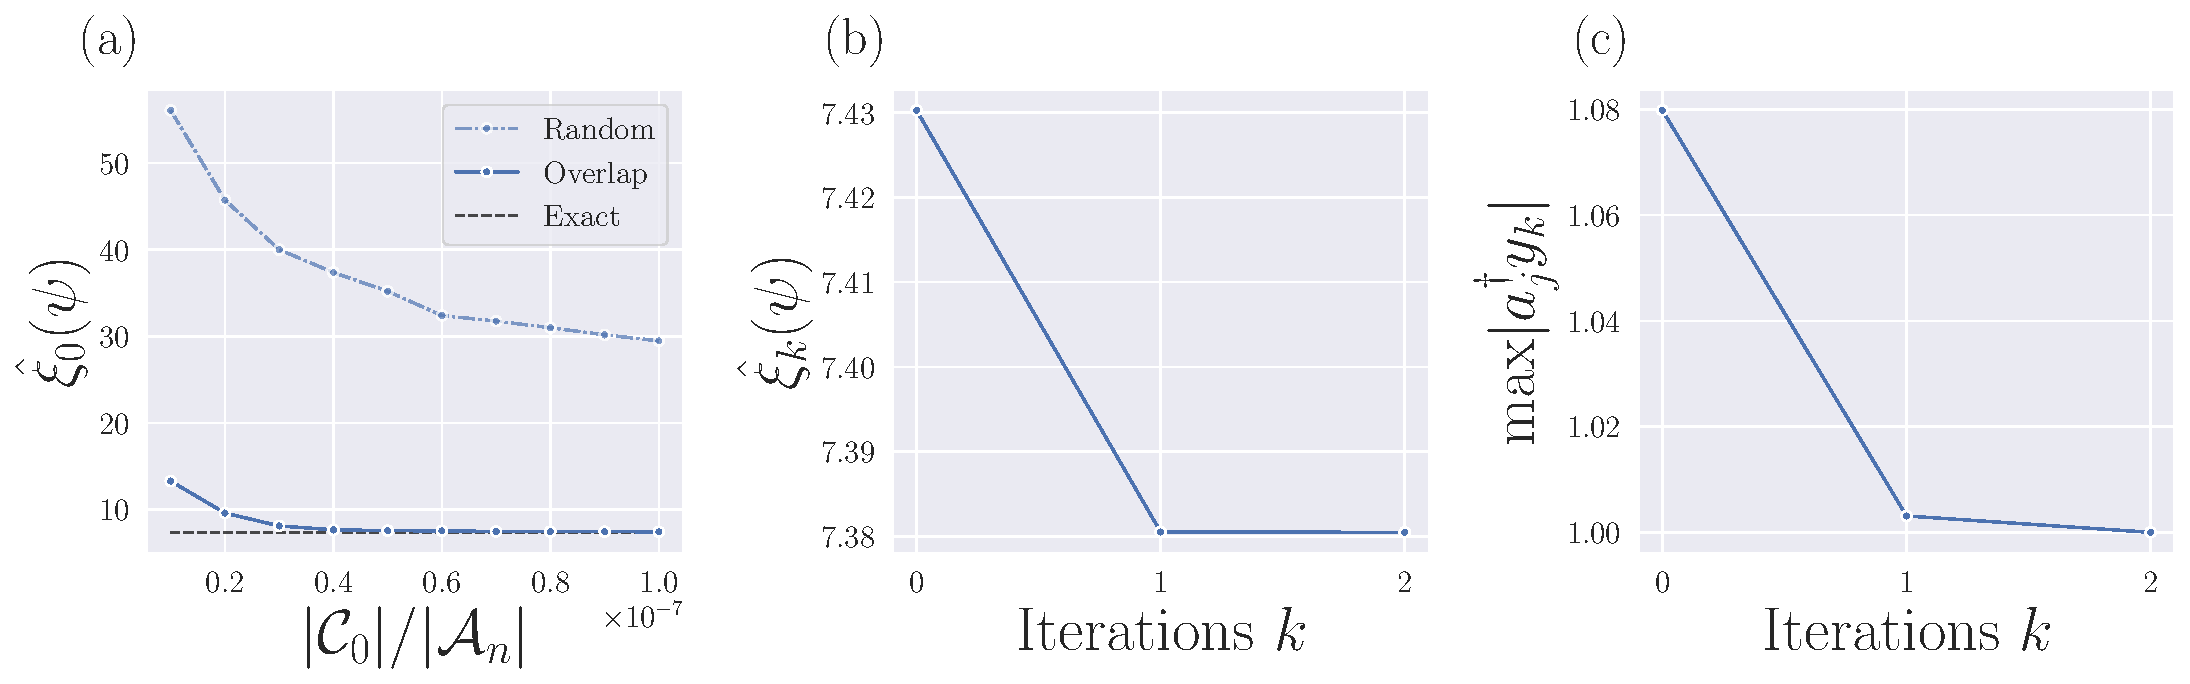
\includegraphics[width=\columnwidth]{../../image/CG_7.pdf}
  \caption{
    (a) $\norm{x_0}_1$ in the Algorithm~\ref{alg:CG},
    which can be obtained from $\texttt{SolveSOCP}(\calC_0, b)$,
    for a random 8-qubit state.
    The ratio $\abs{\calC_0}/\abs{\calA_n}$
    varies from \orange{$10^{-8}$ to $10^{-7}$}.
    We can get much better results
    with the top overlap heuristics
    compared to the random selection of $\calC_0$.
    (b) The convergence of the CG method
    for the same state.
    The max violation becomes 1.00
    after \orange{10} iterations, which means
    the optimal solution is found.
  }
  \label{fig:CG}
\end{figure}

Next, we introduce the CG method
outlined in Algorithm~\ref{alg:CG}.
This iterative algorithm solves
a subproblem restricted to $\calC \subseteq \calA_n$
per each iterations.
It begins with a small subset $\calC_0$
and progressively adds columns $\calC'_k$
that violate the constraints of the dual problem~\eqref{eq:stabilizerExtentDual},
and terminate if there are no more violated columns.
For further implementation details,
we direct the reader
to~\cite{hamaguchiHandbookEfficientlyQuantifying2023},
There are two key aspects of this algorithm:
the initialization process and
the optimality of the solution.
We will discuss these
in subsequent sections.

\subsubsection{Initialization}

In the initial step of Algorithm~\ref{alg:CG},
we select a subset $\{a_j\} = \calC_0 \subseteq \calA_n$
in descending order of $\abs{a_j^\dagger b}$,
which can be computed efficiently
as stated in Theorem~\ref{thm:complexityStabilizerOverlap}.
This heuristic can be justified
by the interpretation of
$\abs{a_j^\dagger b} = \abs{\braket{\phi_j}{\psi}}$
as the "closeness" between the states
$\ket{\psi}$ and $\ket{\phi_j}$.
Hence, choosing the states based on their overlaps
is a reasonable choice.
The numerical experiments result
in~\cite{hamaguchiHandbookEfficientlyQuantifying2023}
also support the effectiveness of this heuristic.
In the case of a random pure 8-qubit state,
even if we use as small subset as $\abs{\calC_0} = 10^{-7} \abs{\calA_n}$,
the $\norm{x_0}_1$ obtained closely approximates the exact value
and outperforms randomly selected $\calC_0$.

\subsubsection{Optimality of the solution}

The terminate criterion for Algorithm~\ref{alg:CG}
is the absence of columns that violate
the dual constraints $\abs{a_j^\dagger y_k} \leq 1$,
which is checked by the subroutine in Section~\ref{sec:coreSubroutine}.
This means the optimal solution for the
dual problem~\eqref{eq:stabilizerExtentDual}
is found, and the primal solution $x_k$ is also optimal
thank to the strong duality of the SOCP problem.
Consequently, we can affirm that
Algorithm~\ref{alg:CG} is certain to
find the exact stabilizer extent
for any $n$-qubit state $\ket{\psi}$
once it terminates.
The convergence of the CG method
is also confirmed in the numerical experiments.
For the same 8-qubit state,
$\max_{a_j \in \calA} \abs{a_j^\dagger y_k}$
reaches 1.00 after 10 iterations,
indicating the discovery of the optimal solution.

\subsection{For the case $\ket{\psi}$ is Real}
\label{sec:restrictedRealProblem}

\begin{figure}[htbp]
  \centering
  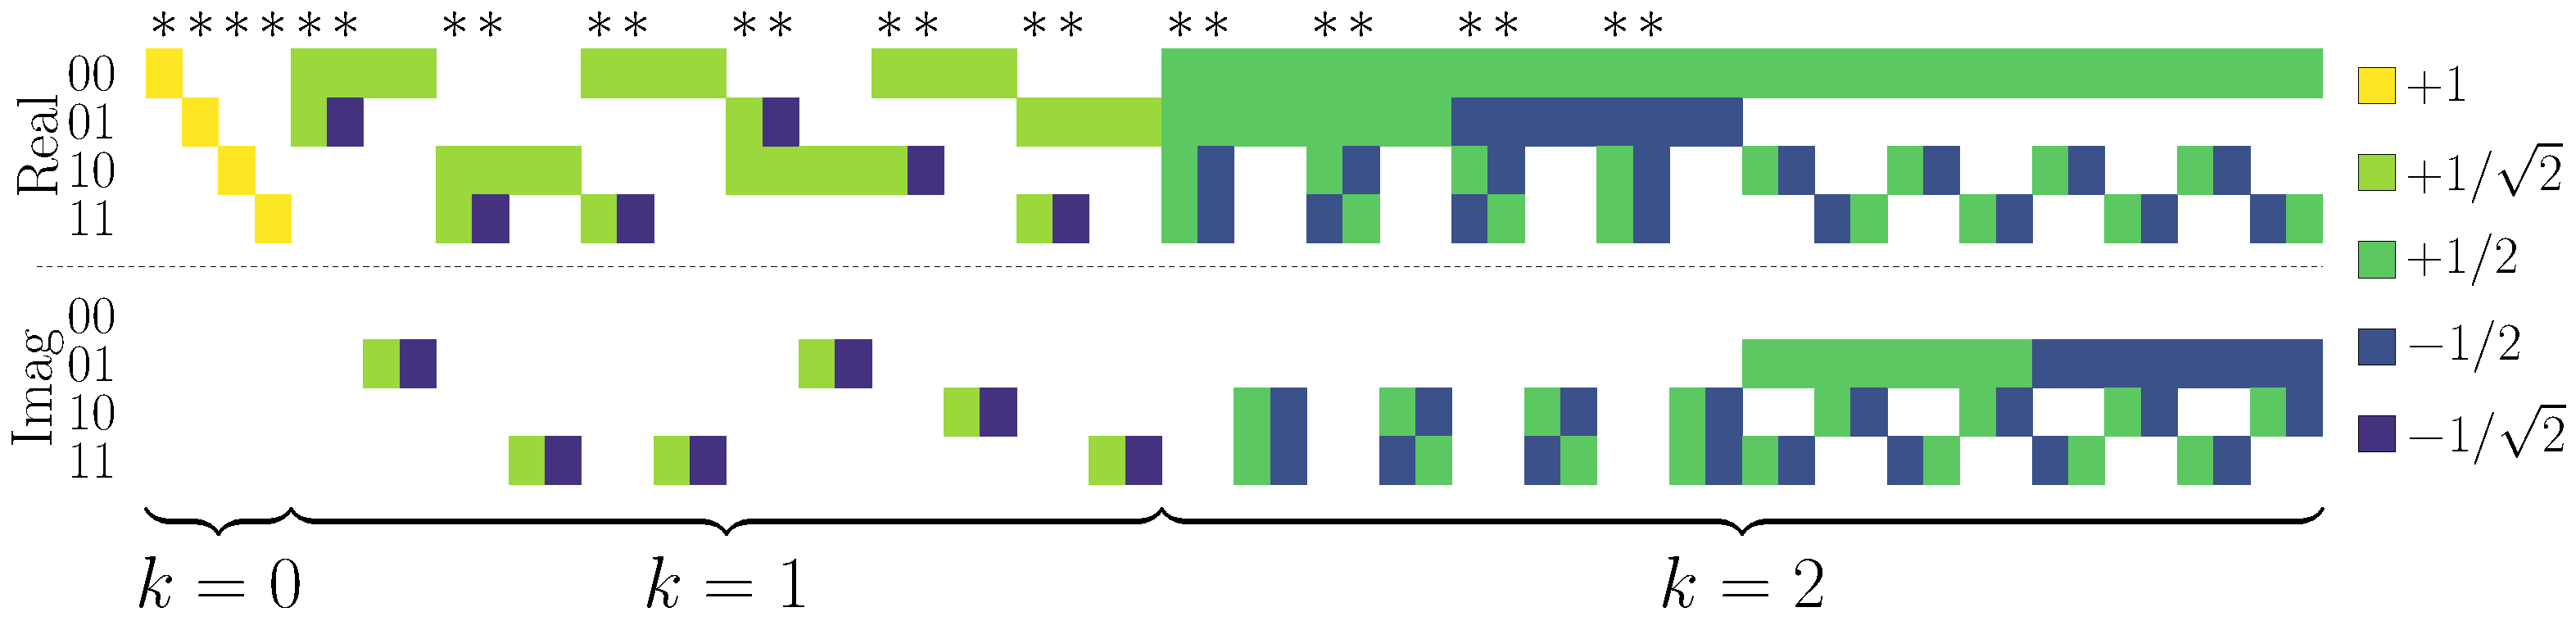
\includegraphics[width=\columnwidth]{imgs/Amat.pdf}
  \caption{
    Visualization of the matrix $A_n$ with $n=2$.
    The upper half corresponds to the real part,
    and the lower half corresponds to the imaginary part.
    The $j$-th column of this represents
    the column $a_j$ and its state $\ket{\phi_j}$.
    The $k$ below the matrix
    corresponds to
    the standard form \eqref{eq:stabilizerStateStandardForm}.
    By restricting the matrix $A_n$
    to the starred columns
    which are real vectors,
    we can obtain the matrix $A_n'$.
  }
  \label{fig:Amat}
\end{figure}

In some cases, the state $\ket{\psi}$ could be real.
For example, ... .
We show that in such cases the problem can be further simplified.
We define the subset of the states in $\calS_n$ with real coefficients as $\calT_n$,
and the corresponding subset of the columns in $\calA_n$ as $\calA'_n$.
Then, the next theorem holds.
\begin{restatable}{theorem}{restrictedRealProblem}
  \label{thm:restrictedRealProblem}
  Suppose that the state $\ket{\psi}$ is real.
  If we substitute the column set $\calA_n$ with $\calA'_n$
  in the problem~\eqref{eq:stabilizerExtentPrimal},
  the optimal solution of the restricted problem
  is also optimal for the original problem.
\end{restatable}

Thanks to theorem~\ref{thm:restrictedRealProblem},
we can reduce the size of the column set size
by a factor of $2^n$.

\section{Approx Solutions}

\section{Discussion}

In this paper, we have shown that \orange{todo}.

There is still room for improvement
in some specific cases.
As for Robustness of Magic,
there is a marvelous algorithm
proposed in~\cite{Heinrich2019robustnessofmagic}
which focuses on copies of symmetric pure magic states,
and we enhanced this result in~\cite{hamaguchiHandbookEfficientlyQuantifying2023}.
Applying such techniques to the stabilizer extent calculation
would be promising and is left for future work.

Furthermore, there is some more future direction.
For example, \orange{todo}.

\emph{Acknowledgements.---}

We would like to thank \orange{N. Marumo} for valuable comments on the manuscript.
\orange{N.Y. wishes to thank JST PRESTO No. JPMJPR2119 and the support
  from IBM Quantum. This work was supported by JST Grant Number JPMJPF2221.
  This work was supported by JST ERATO Grant Number JPMJER2302 and JST CREST
  Grant Number JPMJCR23I4, Japan.}

\bibliographystyle{quantum}
\bibliography{stabilizerExtent}

\appendix

\subfile{APP_impl.tex}

\subfile{APP_real.tex}

\end{document}
